% Template for Cogsci submission with R Markdown

% Stuff changed from original Markdown PLOS Template
\documentclass[10pt, letterpaper]{article}

\usepackage{cogsci}
\usepackage{pslatex}
\usepackage{float}
\usepackage{caption}

% amsmath package, useful for mathematical formulas
\usepackage{amsmath}

% amssymb package, useful for mathematical symbols
\usepackage{amssymb}

% hyperref package, useful for hyperlinks
\usepackage{hyperref}

% graphicx package, useful for including eps and pdf graphics
% include graphics with the command \includegraphics
\usepackage{graphicx}

% Sweave(-like)
\usepackage{fancyvrb}
\DefineVerbatimEnvironment{Sinput}{Verbatim}{fontshape=sl}
\DefineVerbatimEnvironment{Soutput}{Verbatim}{}
\DefineVerbatimEnvironment{Scode}{Verbatim}{fontshape=sl}
\newenvironment{Schunk}{}{}
\DefineVerbatimEnvironment{Code}{Verbatim}{}
\DefineVerbatimEnvironment{CodeInput}{Verbatim}{fontshape=sl}
\DefineVerbatimEnvironment{CodeOutput}{Verbatim}{}
\newenvironment{CodeChunk}{}{}

% cite package, to clean up citations in the main text. Do not remove.
\usepackage{apacite}

% KM added 1/4/18 to allow control of blind submission
\cogscifinalcopy

\usepackage{color}

% Use doublespacing - comment out for single spacing
%\usepackage{setspace}
%\doublespacing


% % Text layout
% \topmargin 0.0cm
% \oddsidemargin 0.5cm
% \evensidemargin 0.5cm
% \textwidth 16cm
% \textheight 21cm

\title{A synthesis of early cognitive and language development using
(meta-)meta-analysis}

\usepackage{booktabs}
\usepackage{longtable}
\usepackage{array}
\usepackage{multirow}
\usepackage{wrapfig}
\usepackage{float}
\usepackage{colortbl}
\usepackage{pdflscape}
\usepackage{tabu}
\usepackage{threeparttable}
\usepackage{threeparttablex}
\usepackage[normalem]{ulem}
\usepackage{makecell}
\usepackage{xcolor}

\author{Anjie Cao$^1$  (anjiecao@stanford.edu), 
 Molley Lewis (mollylewis@gmail.com), \\
 and \bf{Michael C. Frank$^1$ (mcfrank@stanford.edu)} \\
$^1$Department of Psychology, Stanford University }

\newlength{\cslhangindent}
\setlength{\cslhangindent}{1.5em}
\newenvironment{CSLReferences}%
  {}%
  {\par}

\begin{document}

\maketitle

\begin{abstract}
Young children acquire a wide range of linguistic and cognitive skills
in the first three years of life. Decades of experimental work have
established a solid empirical foundation for our understanding of
cognitive development. But most experimental studies are limited in
statistical power and focus on specific psychological constructs, thus
making them unsuitable for describing developmental growth at scale.
Here, we turned to meta-analyses of experimental research. We conducted
a meta-meta-analysis to consolidate and integrate 23 meta-analyses
compiled on MetaLab, a community-augmented meta-analysis platform. We
found that most datasets can not meaningfully distinguish different
functional forms for developmental change, but in those that could,
there is great diversity in the best-fitting functional forms of the age
model. We also evaluated the impact of a range of methodological
factors. Overall, our work sheds light on the heterogeneous nature of
developmental trajectories and the subtle interactions between research
methods and experimental outcomes.

\textbf{Keywords:}
meta-analysis; cognitive development; language learning
\end{abstract}

\hypertarget{introduction}{%
\section{Introduction}\label{introduction}}

In the first three years of life, children undergo a plethora of
developmental changes, transitioning from newborn infants who possess a
limited understanding of language and categories to toddlers who are
able to master a wide range of linguistic and cognitive skills. Despite
a wealth of research examining cognitive development, constructing a
comprehensive theory of cognitive development remains a formidable
challenge. Research in this area generally falls under two categories:
observational research and experimental research. Observational studies
using instruments like the Bayley Scales can provide a holistic picture
of an individual child's development (e.g. Bayley, 2006), but it is a
challenge to move from global developmental milestones to underlying
mechanisms. In contrast, experimental research allows causal tractions
on potential mechanisms, but it typically focuses on one single
construct and does not reveal the connections between different
processes and mechanisms.

In this paper, we aim to provide a quantitative synthesis of
experimental work across multiple areas of developmental psychology,
providing insights into the interrelatedness between psychological
constructs. We achieve this goal by consolidating and integrating 23
meta-analyses of cognitive and language development compiled on MetaLab,
a community-augmented meta-analysis platform.

Statistical meta-analysis, the technique of aggregating effect sizes
across a systematic sample of experiments, has some unique advantages as
a source of data about developmental processes in early childhood. First
and foremost, it allows researchers to explore questions that are
difficult to address with individual studies. One such example is the
functional form of developmental curves, or how different psychological
processes change over time. Many developmental studies use linear
regression models with age as a predictor, but this assumption of
linearity may not capture the complexities of developmental processes.
For example, some cognitive abilities -- such as relational reasoning --
might follow an inverted-U shape (Carstensen et al., 2019; Walker,
Bridgers, \& Gopnik, 2016), while others -- like early vocabulary size
-- show an exponential increase (Frank, Braginsky, Yurovsky, \&
Marchman, 2021). These non-linear trends can be challenging to identify
and interpret with limited data from individual studies, but
meta-analytic methods can provide a large amount of data across a broad
age range, enabling researchers to evaluate and compare different
functional forms of developmental trajectories.

Meta-analysis can also shed light on how research methods influence the
strengths of observed effects. Research methods and theories are
fundamentally intertwined, and this is especially true for developmental
psychology, in which even small changes to the methods could
substantially change the outcomes (Dale, Warlaumont, \& Johnson, 2022).
One example is the influence of familiarization time. It has been
proposed that the amount of exposure infants have prior to the test
events can influence infants' direction of preference (i.e.~novelty
preference or familiarity preference, Hunter \& Ames, 1988). Although
the empirical evidence for this theory is mixed, this ambiguity has
significant downstream consequences on our understanding of infants'
cognitive capabilities (Bergmann \& Cristia, 2016; Cf. Black \&
Bergmann, 2017). Debates about infants' arithmetic competence or their
evaluations of social agents are often centered around the direction of
preferences (Infants arithmetic competence: Clearfield \& Westfahl,
2006; Wakeley, Rivera, \& Langer, 2000; Wynn, 1993; Evaluation of social
agents: Hamlin, Wynn, \& Bloom, 2007; Salvadori et al., 2015). Due to
the time and resources required for developmental studies, it is often
difficult to directly evaluate the impact of subtle changes in methods.
Therefore, meta-analytic methods provide a unique opportunity to
investigate the effects of methodological factors on research findings.

Last but not least, meta-analytic methods make it possible to compare
and connect research findings across research areas. The use of effect
size as the fundamental unit of analysis allows for comparisons across
different domains and research areas. These comparisons can provide
insight into how different processes facilitate learning at different
stages of development and can aid in the development of data-driven
cognitive development theories (Cao \& Lewis, 2022; Lewis et al., 2016).
However, a synthesis across multiple domains requires a database of
multiple meta-analyses. Towards that aim, MetaLab was established to
provide an open database of meta-analyses (Bergmann et al., 2018).
Developmental researchers are invited to deposit their meta-analysis
dataset into MetaLab, and they are encouraged to use the datasets for
custom analyses. As of November 2022, Metalab contains 2,497 effect
sizes from 30 different meta-analyses. This resource allows the
beginnings of a quantitative synthesis across different research areas
in developmental psychology.

In particular, we address three questions. First, we investigate the
shape of developmental curves across domains. The form of growth curves
has been of interest in a lot of areas of developmental research (e.g.,
accelerating growth in vocabulary: McMurray, 2007; asymptotic decreases
in reaction time: Kail, 1991). These nuanced descriptions of
developmental trajectories allow for a more precise understanding of the
mechanisms driving these changes. We aim to provide these quantitative
descriptions for more research areas. Second, we hope to understand how
research methods moderate the strengths of the findings. Increasingly,
developmental research methods are scrutinized for their mechanisms and
scientific rigor (Paulus, 2022; Stahl \& Kibbe, 2022). With MetaLab, the
field is ripe for a more systematic understanding of how different
design choices in experiments could influence the results. Finally, we
offer a birds-eye view of the field by integrating the growth curves
across multiple domains. This view would provide an empirical foundation
for creating a synthesized theory of cognitive development.

\hypertarget{methods}{%
\section{Methods}\label{methods}}

\hypertarget{datasets}{%
\subsubsection{Datasets}\label{datasets}}

Datasets were retrieved from \texttt{metalabr}, the R package built from
Metalab. As of November 2022, the package includes 30 individual
meta-analysis datasets covering different research domains in language
learning and cognitive development. Our current datasets deviate from
the retrieved datasets in the following way: 2 datasets were removed due
data quality issues (Word segmentation neuro: only contained 1 study;
Phonotactic learning: yielded null meta-analytic effect); 3 datasets
were removed due to being observational studies or including studies
with quasi-experimental design (Pointing and vocabulary concurrent;
Pointing and vocabulary, longitudinal; Video deficit); 1 dataset was
replaced with a more updated version (Infant directed speech
preference); 2 pairs of dataset were combined into one because they
measure theoretically identical constructs (Pair 1: Word segmentation
behavioral, Functional word segmentation; Pair 2: Gaze following live,
Gaze following video).

The final dataset contains 23 meta-analyses. Table 1 provides a summary
of the datasets, along with the number of effect sizes and participants
included in each dataset.

The final dataset and analysis scripts are available at
\url{https://tinyurl.com/metalabCogsci}.

\hypertarget{analytic-methods}{%
\subsubsection{Analytic Methods}\label{analytic-methods}}

All analyses were conducted in R using the \texttt{metafor} package
(Viechtbauer, 2010). We specified multi-level random effect models with
random effect structures that included grouping by paper and by
participant group. We removed the clustering if grouping information was
missing from the dataset. All moderators were included as fixed effects.
All model comparisons were based on the corrected Akaike Information
Criterion (AICc).

\hypertarget{results}{%
\section{Results}\label{results}}

\hypertarget{functional-form-of-developmental-curves}{%
\subsection{Functional form of developmental
curves}\label{functional-form-of-developmental-curves}}

\begin{table*}[ht]
\begin{tabular}{l|r|r|l|r|r|r|r}
\hline
\textbf{Dataset} & N ES & N Participants & ES & Const. & Linear & Log & Quad.\\
\hline
Statistical sound category learning  & 11 & 350 & 0.56 [0.19,0.93] & \textbf{0.0*} & 3.0* & 4.1 & 2.5*\\
Vowel discrimination (native) & 143 & 2418 & 0.59 [0.43,0.75] & \textbf{0.0} & 1.3 & 1.0 & 1.6\\
Vowel discrimination (non-native) & 49 & 600 & 0.65 [0.2,1.1] & \textbf{0.0} & 1.6 & 1.7 & 1.5\\
Statistical word segmentation & 103 & 804 & -0.08 [-0.18,0.02] & \textbf{0.0} & 1.3 & 1.5 & 1.1\\
Switch task & 143 & 2764 & -0.16 [-0.25,-0.06] & \textbf{0.0} & 1.1 & 1.1 & 1.1\\
Prosocial agents & 61 & 1244 & 0.4 [0.29,0.52] & \textbf{0.0} & 2.1 & 1.9 & 2.1\\
Simple arithmetic competences & 14 & 369 & 0.25 [0.04,0.46] & \textbf{0.0} & 6.7 & 6.7 & 6.6\\
Symbolic play & 196 & 7148 & 0.63 [0.53,0.72] & \textbf{0.0} & 0.6 & 0.5 & 0.6\\
Word Segmentation  & 315 & 2910 & 0.2 [0.14,0.26] & \textbf{0.0} & 1.3 & 1.0 & 1.6\\
Infant directed speech preference & 83 & 985 & 0.47 [0.28,0.65] & \textbf{0.0} & 1.0 & 1.8 & 0.9\\
Online word recognition & 14 & 330 & 1.37 [0.78,1.96] & 2.2 & \textbf{0.0} & 0.2 & 0.1\\
Mutual exclusivity & 131 & 2222 & 1.27 [0.99,1.56] & 37.2 & 5.8 & \textbf{0.0*} & 16.9\\
Label advantage in concept learning & 100 & 1644 & 0.36 [0.23,0.48] & 2.4 & 0.9 & \textbf{0.0} & 1.6\\
Sound symbolism & 44 & 425 & 0.16 [-0.01,0.33] & 2.9 & 0.0 & \textbf{0.0} & 0.7\\
Categorization bias & 80 & 382 & 0.25 [-0.54,1.05] & 0.9 & 0.3 & \textbf{0.0} & 0.4\\
Syntactic bootstrapping & 60 & 832 & 0.24 [0.03,0.44] & 0.5 & 0.3 & \textbf{0.0} & 0.6\\
Mispronunciation sensitivity & 249 & 2122 & 0.45 [0.24,0.66] & 30.7 & 6.4 & 14.5 & \textbf{0.0*}\\
Cross-situational word learning & 48 & 2241 & 0.67 [0.5,0.84] & 4.0 & 0.1* & 1.9* & \textbf{0.0*}\\
Gaze following  & 81 & 1407 & 0.81 [0.61,1.01] & 43.7 & 2.1* & 10.4 & \textbf{0.0*}\\
Familiar word recognition & 34 & 586 & 0.54 [0.38,0.69] & 1.7 & 0.3 & 1.1 & \textbf{0.0}\\
Abstract rule learning & 95 & 1123 & 0.22 [0.07,0.37] & 0.4 & 0.3 & 0.9 & \textbf{0.0}\\
Natural speech preference & 55 & 786 & 0.44 [0.23,0.65] & 0.9 & 0.4 & 1.0 & \textbf{0.0}\\
Language discrimination and preference & 153 & 2060 & -0.13 [-0.26,0] & 2.3 & 2.0 & 2.9 & \textbf{0.0}\\


\hline
\end{tabular}
\caption{\label{demo-table}This table summarizes the number of effect sizes \(ES\) and the number of participants included in each meta-analysis dataset. The ES estimates represent the aggregated effect sizes and their 95\% confidence intervals from each dataset. The last four columns include the values of $\Delta_{i}$ of corrected Akaike Information Criterion \(AICc\) for the age model with different functional forms: Constant, Linear, Logarithmic, and Quadratic. The values were calculated from subtracting the minimum AICc from the AICc of each model. They were rounded to one decimal. The bold values represent the smallest values among the four functional forms before rounding. Asterisks mark the models that are significantly better than the other models in the same research area.}
\end{table*}

Our first research question was about the functional form of the
developmental trajectories we observed. We considered four specific
forms: constant, linear, logarithmic, and, quadratic, each considered as
an age-related fixed effect. We evaluated the models based on corrected
AICc (Table 1).

When using AICc in model selection, the value needs to be contextualized
in relation to the lowest AICc. Under the conventional interpretation,
\(\Delta_{i}\) (\(AIC_i - AIC_{min}\), where \(AIC_i\) is the model
being evaluated, and \(AIC_{min}\) is the lowest AIC among the set of
models) less than 4 suggests minimal evidence against the model with
higher AICc; \(\Delta_{i}\) above 4 suggests substantial support for the
model with lower AICc (Burnham \& Anderson, 2004). With this
interpretation framework, the functional forms in most domains can not
be meaningfully distinguished, with exceptions in 6 domains. In Mutual
Exclusivity, there is a strong preference for the logarithmic model
(\(\Delta_{Linear}\) = 5.75 ; \(\Delta_{Quad.}\) = 16.91;
\(\Delta_{Const.}\) = 37.21). We also found a strong preference for the
quadratic model in Mispronunciation sensitivity (\(\Delta_{Linear}\) =
6.39; \(\Delta_{Log}\) = 14.49; \(\Delta_{Const.}\) = 30.74) and a
strong preference for the constant model in Simple arithmetic competence
( \(\Delta_{Quad.}\) = 6.55;\(\Delta_{Linear}\) = 6.65; \(\Delta_{Log}\)
= 6.74). The comparison is less clear-cut in Gaze following, where there
is support for the Quadratic model against the Constant model and the
Logarithmic model (\(\Delta_{Log}\) = 10.41;\(\Delta_{Const.}\) =
43.73), but the Linear model is comparable with the Quadratic model
(\(\Delta_{Linear}\) = 2.07). Finally, in Statistical sound category
learning and Cross situational word learning, we only found evidence
against the logarithmic model (\(\Delta_{Log}\) = 4.08) and the constant
model (\(\Delta_{Log}\) = 4.01), respectively.

\hypertarget{methodological-moderators}{%
\subsection{Methodological Moderators}\label{methodological-moderators}}

In this section, we considered methodological moderators shared by
multiple datasets. Given the limited number of studies conducted with
neuroimaging methods, we focused our analyses on studies conducted with
behavioral methods. Therefore, we excluded studies that were conducted
with either fNIRS or EEG. Moreover, to minimize age-related
heterogeneity, we only included studies with participants' mean age
below 36 months. All analyses were conducted on the subset of research
domains with multiple levels for the moderator of interests. Figure 1
provides a summary of the estimates for moderators.

\begin{CodeChunk}
\begin{figure*}[t!]

{\centering 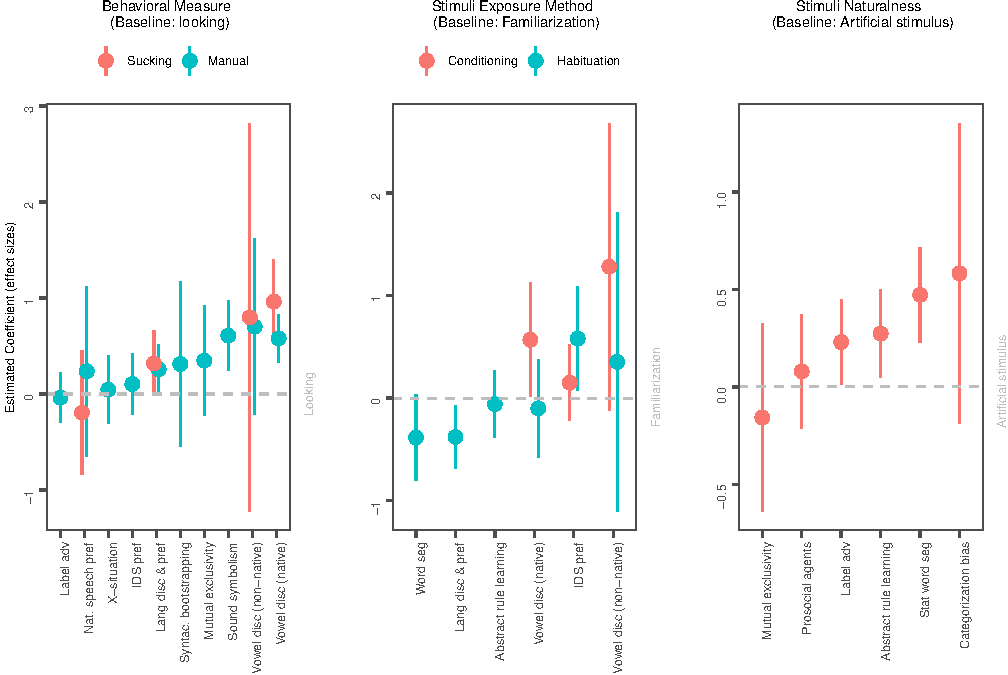
\includegraphics{figs/mod_plot-1} 

}

\caption[Each panel shows the moderator estimates]{Each panel shows the moderator estimates. Each dot represents the estimate of the particular moderator level compared to the baseline. For behavioral measure, the baseline level is looking. Red dots indicate the estimate for studies using sucking measure, and the teal dots indicate the estimates for studies using manual measure. For stimuli exposure method, the baseline level is familiarization. Red, and teal represent the estimates for studies using conditioning and habituation in exposure phase, respectively. For stimuli naturalness, the dots represent the estimate for studies using natural stimuli (e.g. real-world objects; natural speech) compared to studies using artificial stimuli (e.g. pictures, synthetic speech). Error bars show 95\% confidence intervals.}\label{fig:mod_plot}
\end{figure*}
\end{CodeChunk}

\hypertarget{behavioral-measures}{%
\subsubsection{Behavioral Measures}\label{behavioral-measures}}

Meta-analyses have very heterogeneous moderators coded, but many
included coding of which behavioral response measure was used in the
original study: looking-based behaviors (e.g., looking time or other
eye-tracking measures), sucking (as in the high amplitude sucking
procedure), and manual behaviors (e.g., pointing, exploration). We thus
added behavioral measure as an additional fixed effect to the age model
with the best-fitting functional form from the previous analysis.

In general, nearly all effects were weakly positive such that sucking
and manual response modes yielded slightly larger effect sizes, though
these effects were not always significant. Behavioral measure was a
significant predictor of effect sizes in only two domains, Vowel
Discrimination (Native) and Sound Symbolism. In Vowel Discrimination
(native), studies with Manual or Sucking behavioral measure has larger
effect sizes than studies using looking as the behavioral measure
(Manual: \(\beta\) = 0.58 {[}0.33, 0.82{]}, \emph{z} = 4.6, \emph{p}
\textless{} 0.01; Sucking: \(\beta\) = 0.96 {[}0.53, 1.4{]}, \emph{z} =
4.34, \emph{p} \textless{} 0.01). Similarly, in Sound Symbolism, studies
with manual behavioral measures also yield larger effect sizes than
looking studies (\(\beta\) = 0.61 {[}0.24, 0.97{]}, \emph{z} = 3.29,
\emph{p} \textless{} 0.01).

We also explored whether there would be an interaction between the
research method and participants' age. The inclusion of interaction
terms did not meaningfully improve the AICc of any of the main model
(All \(\Delta_{interaction}\) \textless{} 2). The current datasets can
not distinguish between the interaction effect and the main effect.

\hypertarget{stimuli-exposure-method}{%
\subsubsection{Stimuli Exposure Method}\label{stimuli-exposure-method}}

Stimuli exposure method refers to the type of exposure infants have
during the experiments prior to the test events. There are typically
three types of stimuli exposure method: 1) an infant would be
conditioned to show an orienting behavior (conditioning); 2) an infant
would be exposed to a stimulus for a constant amount of time
(familiarization); 3) an infant would be shown some stimulus repeatedly
until the magnitude of response drops below a threshold (habituation).
We coded these three types of stimuli exposure methods as three levels
in the moderator stimuli exposure method.

Stimuli exposure method is a significant predictor of effect sizes in
three domains. In Vowel discrimination (native), conditioning studies
yielded larger effect sizes than familiarization studies (\(\beta\) =
0.57 {[}0.01, 1.12{]}, \emph{z} = 2.01, \emph{p} = 0.04).

The results of the comparison between familiarization studies and
habituation studies are mixed. In Infant directed speech preference,
habituation studies produced larger effect sizes than the
familiarization studies (\(\beta\) = 0.58 {[}0.07, 1.09{]}, \emph{z} =
2.24, \emph{p} = 0.03), whereas the opposite pattern was found in
Language discrimination and preference: habituation studies had smaller
effect sizes than the familiarization studies (\(\beta\) = -0.38
{[}-0.69, -0.07{]}, \emph{z} = -2.41, \emph{p} = 0.02)

\hypertarget{stimuli-naturalness}{%
\subsubsection{Stimuli Naturalness}\label{stimuli-naturalness}}

Next, we considered the effect of stimuli type. We focused on one key
dimension: naturalness. For primarily visual stimuli, we considered
``natural'' to mean stimuli that use real-world objects (e.g.~puppets,
blocks). We compared these natural stimuli with representation-type
stimuli, such as pictures, videos, or drawings. In primarily auditory
stimuli, we compared recorded natural speech with synthesized stimuli.

Natural stimuli has advantages over artificial stimuli across
modalities. We found that naturalness was a significant predictor for
Label advantage in concept learning, with natural stimuli yielding
larger effect sizes than representation-type stimuli (\(\beta\) = 0.23
{[}0.01, 0.45{]}, \emph{z} = 2.06, \emph{p} = 0.04). Similarly, in both
Statistical word segmentation and Abstract rule learning, we found a
natural speech advantage (Statistical word segmentation: \(\beta\) =
0.47 {[}0.23, 0.72{]}, \emph{z} = 3.8, \emph{p} \textless{} 0.01;
Abstract rule learning: \(\beta\) = 0.27 {[}0.05, 0.5{]}, \emph{z} =
2.35, \emph{p} = 0.02).

\hypertarget{major-author}{%
\subsubsection{Major author}\label{major-author}}

Margoni \& Surian (2018) found evidence for an author-based bias in the
prosocial agents literature: results produced by certain authors were
consistently larger. We evaluated how prevalent this phenomenon was in
the literature by coding a ``major author'' moderator. Authors are
considered to be a ``major author'' if they are listed as authors in
more than 15\% of the papers in the research area. When multiple major
authors co-authored the same set of publications, we considered one
author from that author group. When multiple authors were considered as
major authors but were associated with different publications, we
selected the ones with the most publications in the research area.

We found evidence for a major author effect in 8 datasets, where studies
produced by the major author were larger than the rest of the papers. In
3 datasets, however, we also found the opposite patterns, where certain
authors produced on average smaller effect sizes than the rest of the
literature.

\begin{CodeChunk}
\begin{figure}[t!]

{\centering 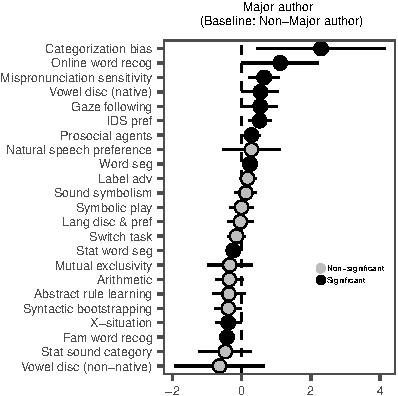
\includegraphics{figs/image-1} 

}

\caption[Each dot represents the estimate for studies produced by major author in the particular research area, compared to other studies in the same research area]{Each dot represents the estimate for studies produced by major author in the particular research area, compared to other studies in the same research area. Error bars show 95\% confidence intervals. }\label{fig:image}
\end{figure}
\end{CodeChunk}

\hypertarget{synthesis}{%
\subsection{Synthesis}\label{synthesis}}

Finally, we synthesized all 23 datasets by grouping them based on the
type of theoretical constructs they represented: Cognitive abilities,
Communication, Sounds, and Words. We integrated the predictions from the
best-fitting age-based models in Figure 2, showing predictions across
the range of measured ages (See SI for each prediction line along with
the corresponding data). We found a striking range of functional forms
in the developmental trajectories across all types of theoretical
constructs. In particular, the magnitudes of some phenomena -- online
word recognition, gaze following, and mutual exclusivity, for example --
increased substantially over development. In contrast, others -- sound
symbolism, categorization bias, and others -- stayed constant at a
measurable level without showing developmental increases. We considered
several explanations for why some phenomena would be constant: one is
that these meta-analyses might correspond to relatively more
experience-independent biases. On the other hand, we cannot rule out
cross-experiment confounding wherein experimenters test progressively
harder stimuli with development, thus counteracting any developmental
gains that might otherwise be measured.

\hypertarget{discussion}{%
\section{Discussion}\label{discussion}}

How can we quantitatively describe developmental growth at scale?
Meta-analysis is one promising method. In this paper, we presented a
bird-eye view of developmental psychology by synthesizing 23
meta-analyses available on MetaLab. We found great diversity in the
shapes of the best-fitting models for each domain -- while some
phenomena showed larger and larger effects with development, quite a
number of others stayed constant, suggesting a distinction between small
but measurable in-lab effects and behaviors that can easily be observed
in individual children (effect sizes \textgreater{} 2). We also
considered the moderating effects of different methodological factors,
including the type of behavioral measure, the type of exposure phase,
stimuli naturalness, and whether the work is done by a ``major author''.
These factors moderate effect sizes from different domains in
heterogeneous ways, though we did find evidence for naturalistic stimuli
leading to larger effects in a number of studies.

\begin{CodeChunk}
\begin{figure*}[h!]

{\centering 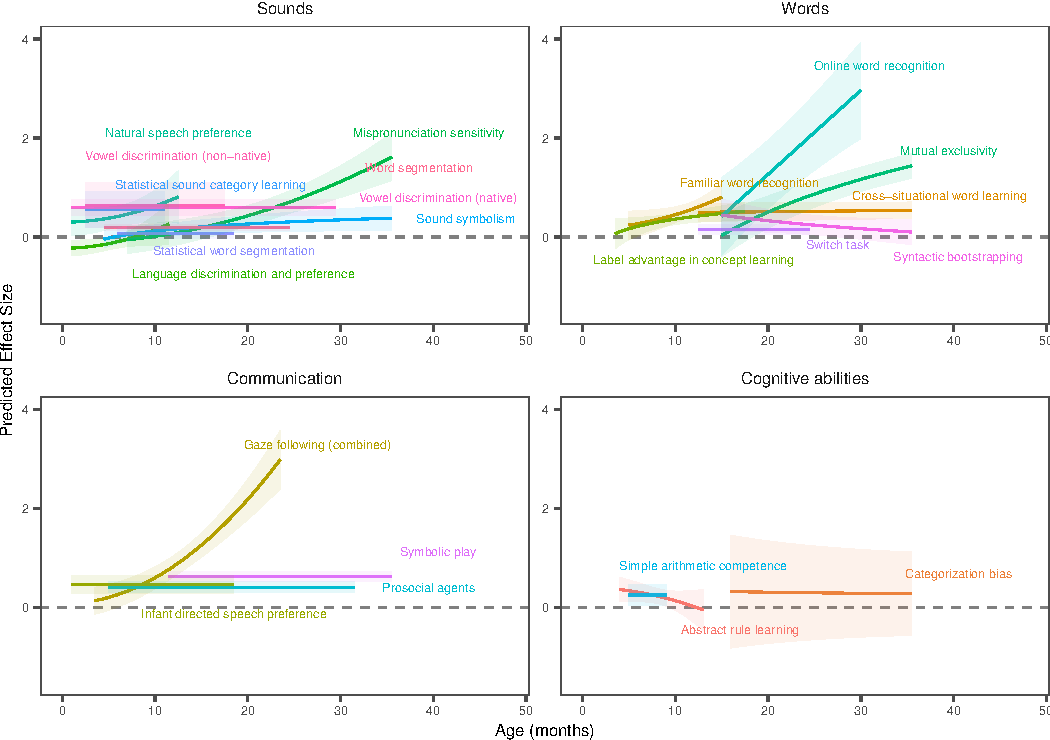
\includegraphics{figs/2-col-imageb-1} 

}

\caption[Predictions of the best-fitting functional forms of the age model]{Predictions of the best-fitting functional forms of the age model. X-axis is age in months. Y-axis is the predicted effect size. For each research area, we plotted the predicted values for the age range included in the dataset.}\label{fig:2-col-imageb}
\end{figure*}
\end{CodeChunk}

This current synthesis highlights the variation in developmental
trajectories, challenging the traditional ``milestone'' view of
cognitive development. Under the milestone view, infants would acquire
different cognitive and linguistic skills as they grow (Meylan \&
Bergelson, 2022; Wilks, Gerber, \& Erdie-Lalena, 2010). Our findings
suggest that this view is missing two important details. First, at any
given age, psychological constructs could have a wide range of effect
sizes. For example, at 20 months of age, the predicted effect sizes for
communication skills range from 0.16 (Switch task) to 2.18 (Gaze
following). The differences between the strengths of the effect may
reflect the differences in how these skills contribute to communication,
with some playing a more significant role than others. In addition, the
development of these skills could follow significantly different
trajectories, with some increasing exponentially with age and others
staying constant throughout early childhood. The heterogeneity of the
developmental process calls for developing a more nuanced and integrated
developmental theory.

The heterogeneity can also partly be attributed to the wide variety of
research methods. In the current analysis, we focused on in-lab
experimental work, and thus the effect sizes may as well reflect how
well the research methods capture the phenomenon of interest. Indeed, we
have shown that subtle experimental procedure changes (e.g.~stimuli
exposure methods) could significantly alter the effect sizes. Moreover,
methods' impact varies across domains, with some domains being more
susceptible to methodological factors than others. Therefore, the
developmental trajectories that we document could be influenced by
researchers adapting their methods to participants of different ages.
Our findings call attention to the importance of understanding methods'
nuances: rather than treating methods as a perfect mirror perfectly
reflecting the phenomenon, they should be regarded as an imperfect lens
that could distort our perception of the phenomenon.

Of course, meta-analysis is not a perfect tool either. Despite the
inclusion of a variety of moderators, we can explain relatively
variation in the datasets. One measure of heterogeneity is \(I^2\),
which calculates the proportion of variance accounted for by the
meta-analytic model, relative to the total variance in the dataset. The
mean \(I^2\) across all the models we ran was 0.74 (\emph{SD} : 0.19),
indicating that the majority of the variation in effects across studies
was unexplained by our moderators (Higgins \& Thompson, 2002).

Moreover, meta-analytic methods can often produce effect sizes
significantly larger than a comparable large-scale replication (Kvarven,
Strømland, \& Johannesson, 2020). Part of the discrepancy can be
attributed to the heterogeneity of research methods that are often
minimized in a large-scale replication (Lewis, Mathur, VanderWeele, \&
Frank, 2020). While we have included methodological moderators in our
analysis, it is highly likely that the coded moderators did not fully
reflect the subtlety of research methods. However, the ``Major author''
effect found in many research domains could provide a window into
understanding the subtler aspects of research methods. In the future, we
could compare and contrast the methods and materials used by ``major
authors'' and those by others. Doing so would allow us to pinpoint the
differences and understand which aspects of the methods really matter,
and which do not.

Our ultimate goal is to offer a data-driven synthetic theory of
cognitive development. Here we have made our first step toward that goal
by offering a synthesis of meta-analyses across 23 different research
domains. Moving forward, we aim to expand and refine our synthesis by
including more research areas, correcting potential publication biases,
and accounting for more detailed methodological factors. We would also
like to make more connections between our meta-analysis-based work and
the many ongoing analyses based on large-scale multi-site replication
projects (e.g.~ManyBabies: Frank et al., 2017). Ultimately, we hope our
analysis can provide a solid empirical foundation to help us to better
understand the complex and diverse processes involved in cognitive
development.

\hypertarget{references}{%
\section{References}\label{references}}

\setlength{\parindent}{-0.1in} 
\setlength{\leftskip}{0.125in}

\noindent

\hypertarget{refs}{}
\begin{CSLReferences}{1}{0}
\leavevmode\vadjust pre{\hypertarget{ref-bayley2006bayley}{}}%
Bayley, N. (2006). Bayley scales of infant and toddler development.

\leavevmode\vadjust pre{\hypertarget{ref-bergmann2016development}{}}%
Bergmann, C., \& Cristia, A. (2016). Development of infants'
segmentation of words from native speech: A meta-analytic approach.
\emph{Developmental Science}, \emph{19}(6), 901--917.

\leavevmode\vadjust pre{\hypertarget{ref-bergmann2018promoting}{}}%
Bergmann, C., Tsuji, S., Piccinini, P. E., Lewis, M. L., Braginsky, M.,
Frank, M. C., \& Cristia, A. (2018). Promoting replicability in
developmental research through meta-analyses: Insights from language
acquisition research. \emph{Child Development}, \emph{89}(6),
1996--2009.

\leavevmode\vadjust pre{\hypertarget{ref-black2017quantifying}{}}%
Black, A., \& Bergmann, C. (2017). Quantifying infants' statistical word
segmentation: A meta-analysis. In \emph{39th annual meeting of the
cognitive science society} (pp. 124--129). Cognitive Science Society.

\leavevmode\vadjust pre{\hypertarget{ref-burnham2004multimodel}{}}%
Burnham, K. P., \& Anderson, D. R. (2004). Multimodel inference:
Understanding AIC and BIC in model selection. \emph{Sociological Methods
\& Research}, \emph{33}(2), 261--304.

\leavevmode\vadjust pre{\hypertarget{ref-cao2022quantifying}{}}%
Cao, A., \& Lewis, M. (2022). Quantifying the syntactic bootstrapping
effect in verb learning: A meta-analytic synthesis. \emph{Developmental
Science}, \emph{25}(2), e13176.

\leavevmode\vadjust pre{\hypertarget{ref-carstensen2019context}{}}%
Carstensen, A., Zhang, J., Heyman, G. D., Fu, G., Lee, K., \& Walker, C.
M. (2019). Context shapes early diversity in abstract thought.
\emph{Proceedings of the National Academy of Sciences}, \emph{116}(28),
13891--13896.

\leavevmode\vadjust pre{\hypertarget{ref-clearfield2006familiarization}{}}%
Clearfield, M. W., \& Westfahl, S. M.-C. (2006). Familiarization in
infants' perception of addition problems. \emph{Journal of Cognition and
Development}, \emph{7}(1), 27--43.

\leavevmode\vadjust pre{\hypertarget{ref-dale2022fundamental}{}}%
Dale, R., Warlaumont, A. S., \& Johnson, K. L. (2022). The fundamental
importance of method to theory. \emph{Nature Reviews Psychology}, 1--12.

\leavevmode\vadjust pre{\hypertarget{ref-frank2017collaborative}{}}%
Frank, M. C., Bergelson, E., Bergmann, C., Cristia, A., Floccia, C.,
Gervain, J., et al.others. (2017). A collaborative approach to infant
research: Promoting reproducibility, best practices, and
theory-building. \emph{Infancy}, \emph{22}(4), 421--435.

\leavevmode\vadjust pre{\hypertarget{ref-frank2021variability}{}}%
Frank, M. C., Braginsky, M., Yurovsky, D., \& Marchman, V. A. (2021).
\emph{Variability and consistency in early language learning: The
wordbank project}. MIT Press.

\leavevmode\vadjust pre{\hypertarget{ref-hamlin2007social}{}}%
Hamlin, J. K., Wynn, K., \& Bloom, P. (2007). Social evaluation by
preverbal infants. \emph{Nature}, \emph{450}(7169), 557--559.

\leavevmode\vadjust pre{\hypertarget{ref-higgins2002quantifying}{}}%
Higgins, J. P., \& Thompson, S. G. (2002). Quantifying heterogeneity in
a meta-analysis. \emph{Statistics in Medicine}, \emph{21}(11),
1539--1558.

\leavevmode\vadjust pre{\hypertarget{ref-hunter1988multifactor}{}}%
Hunter, M. A., \& Ames, E. W. (1988). A multifactor model of infant
preferences for novel and familiar stimuli. \emph{Advances in Infancy
Research}.

\leavevmode\vadjust pre{\hypertarget{ref-kail1991developmental}{}}%
Kail, R. (1991). Developmental change in speed of processing during
childhood and adolescence. \emph{Psychological Bulletin}, \emph{109}(3),
490.

\leavevmode\vadjust pre{\hypertarget{ref-kvarven2020comparing}{}}%
Kvarven, A., Strømland, E., \& Johannesson, M. (2020). Comparing
meta-analyses and preregistered multiple-laboratory replication
projects. \emph{Nature Human Behaviour}, \emph{4}(4), 423--434.

\leavevmode\vadjust pre{\hypertarget{ref-lewis2016quantitative}{}}%
Lewis, M., Braginsky, M., Tsuji, S., Bergmann, C., Piccinini, P. E.,
Cristia, A., et al. (2016). A quantitative synthesis of early language
acquisition using meta-analysis.

\leavevmode\vadjust pre{\hypertarget{ref-lewis2020puzzling}{}}%
Lewis, M., Mathur, M., VanderWeele, T., \& Frank, M. C. (2020). The
puzzling relationship between multi-lab replications and meta-analyses
of the rest of the literature.

\leavevmode\vadjust pre{\hypertarget{ref-margoni2018infants}{}}%
Margoni, F., \& Surian, L. (2018). Infants' evaluation of prosocial and
antisocial agents: A meta-analysis. \emph{Developmental Psychology},
\emph{54}(8), 1445.

\leavevmode\vadjust pre{\hypertarget{ref-mcmurray2007defusing}{}}%
McMurray, B. (2007). Defusing the childhood vocabulary explosion.
\emph{Science}, \emph{317}(5838), 631--631.

\leavevmode\vadjust pre{\hypertarget{ref-meylan2022learning}{}}%
Meylan, S. C., \& Bergelson, E. (2022). Learning through processing:
Toward an integrated approach to early word learning. \emph{Annual
Review of Linguistics}, \emph{8}, 77--99.

\leavevmode\vadjust pre{\hypertarget{ref-paulus2022should}{}}%
Paulus, M. (2022). Should infant psychology rely on the
violation-of-expectation method? Not anymore. \emph{Infant and Child
Development}, \emph{31}(1), e2306.

\leavevmode\vadjust pre{\hypertarget{ref-salvadori2015probing}{}}%
Salvadori, E., Blazsekova, T., Volein, A., Karap, Z., Tatone, D.,
Mascaro, O., \& Csibra, G. (2015). Probing the strength of infants'
preference for helpers over hinderers: Two replication attempts of
hamlin and wynn (2011). \emph{PloS One}, \emph{10}(11), e0140570.

\leavevmode\vadjust pre{\hypertarget{ref-stahl2022great}{}}%
Stahl, A. E., \& Kibbe, M. M. (2022). Great expectations: The construct
validity of the violation-of-expectation method for studying infant
cognition. \emph{Infant and Child Development}, \emph{31}(6), e2359.

\leavevmode\vadjust pre{\hypertarget{ref-viechtbauer2010conducting}{}}%
Viechtbauer, W. (2010). Conducting meta-analyses in r with the metafor
package. \emph{Journal of Statistical Software}, \emph{36}(3), 1--48.

\leavevmode\vadjust pre{\hypertarget{ref-wakeley2000can}{}}%
Wakeley, A., Rivera, S., \& Langer, J. (2000). Can young infants add and
subtract? \emph{Child Development}, \emph{71}(6), 1525--1534.

\leavevmode\vadjust pre{\hypertarget{ref-walker2016early}{}}%
Walker, C. M., Bridgers, S., \& Gopnik, A. (2016). The early emergence
and puzzling decline of relational reasoning: Effects of knowledge and
search on inferring abstract concepts. \emph{Cognition}, \emph{156},
30--40.

\leavevmode\vadjust pre{\hypertarget{ref-wilks2010developmental}{}}%
Wilks, T., Gerber, R. J., \& Erdie-Lalena, C. (2010). Developmental
milestones: Cognitive development. \emph{Pediatrics in Review},
\emph{31}(9), 364--367.

\leavevmode\vadjust pre{\hypertarget{ref-wynn1993erratum}{}}%
Wynn, K. (1993). Erratum: Addition and subtraction by human infants.
\emph{Nature}, \emph{361}(6410), 374--374.

\end{CSLReferences}

\bibliographystyle{apacite}


\end{document}
